\documentclass[11pt]{article}
\usepackage[margin=0.78in]{geometry}
\usepackage{fontspec}
\setmainfont{Latin Modern Roman}
\usepackage{graphicx,booktabs,hyperref,url}
\hypersetup{colorlinks=true,linkcolor=blue,urlcolor=blue}
\sloppy
\urlstyle{tt}
\title{N83 Fixed-Base First-Fall Panel: 144 Systems}
\author{Candidate PDP V2 run report}
\date{2026-11-02}
\begin{document}
\maketitle
\section*{Observed outcome}
The frozen V2 first-fall procedure produced and freshly replayed certificates for all 144 pre-existing fixed-base systems across spike35--spike37, $m=2$--$9$, Koblitz/binary/prime families, and planted/natural targets. The one certificate from the original attempt is preserved separately after its runner raised an exception; the continuation completed the other 143 cases. The independent analyzer reports 143/143 attempt-02 certificates hashed and bound, 143/143 fresh replays, and no problems. The recovered attempt-01 certificate has a successful independent fresh replay and matching S3 readback hash.

The first attempt's producer exit code and stdout/stderr were not captured before the replay-helper exception. That process outcome remains unknown; the certificate itself is present, hash-matched to S3, and replay-verified. The continuation recorded no failed or timed-out native cases.

\section*{Counts and outcomes}
\begin{center}
\begin{tabular}{lrr}
\toprule
Family & Exact first-fall degree 2 & Lower bound $\geq 5$ (exact not found)\\
\midrule
Koblitz & 48 & 0\\
Binary & 48 & 0\\
Prime & 0 & 48\\
\midrule
Total & 96 & 48\\
\bottomrule
\end{tabular}
\end{center}
Each family/$m$ cell contains six systems ($3$ candidate IDs $\times$ $2$ target kinds), for $m=2,\ldots,9$. The plot shows recorded counts per cell; it does not estimate a population parameter.

\begin{center}
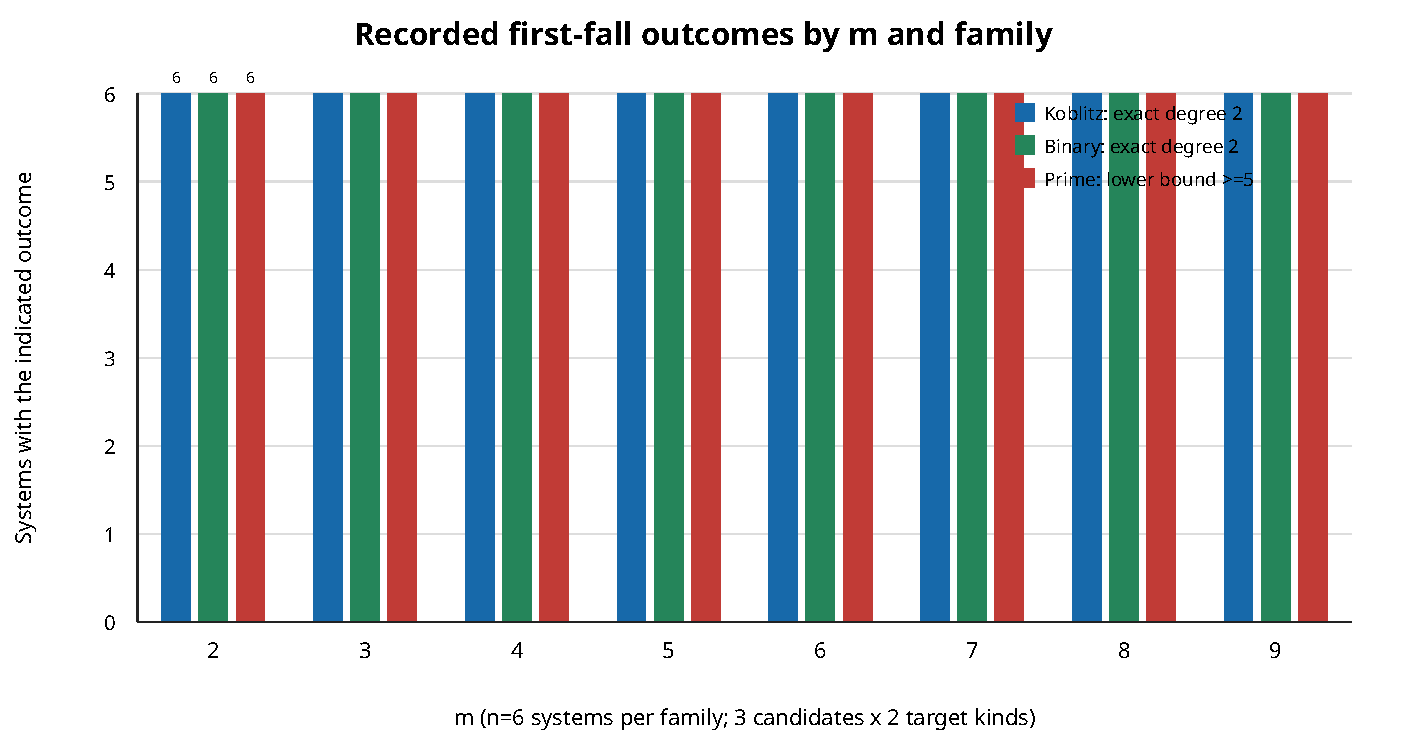
\includegraphics[width=0.73\linewidth]{plot.pdf}
\end{center}

\section*{Protocol and execution}
Protocol: \url{N83-FACTOR-BASE-PDP-FFD-LFD-20261031-V2}, frozen digest \url{50cd6f8213789de2dfd54a3b33a067ed87cc0def761b7c98769be3e19aee47a9}. Inputs were the existing 144 fixed-base systems (fixed candidate x-domain $2^{27}$), not regenerated. Each case was sequential, bounded to 60 seconds and 8 GiB, with a fresh-process certificate replay.

The continuation was launched with \texttt{python3}, script \path{research/n83_candidate_pdp_20261028/evidence/n83-factorbase-variants/candidate-fall-20261102/attempt-02/run_remaining.py}, and argument \texttt{--run}. Per-case commands are preserved in each \texttt{attempt.json}; they invoke the pinned release binary \texttt{fall run} and then \texttt{fall replay}. The attempt-02 runner and analyzer hashes are in \url{attempt-02/script-binding.json}. Pre-data source commit: \url{16c0ed20cb0f625367af79fde27f76600fa88bc6}. Execution host: \url{ip-172-31-26-169.us-east-2.compute.internal}, Linux x86\_64.

Across the 143 continuation cases, recorded producer process elapsed time sums to 314.742 s (median 1.502 s, range 0.740--27.215 s). Recorded replay process elapsed time sums to 89.001 s (median 0.285 s, range 0.006--3.220 s). These are sums of per-case wall-clock durations, not CPU time or end-to-end campaign wall time. Attempt-01's producer duration was not captured.

\section*{Interpretation and next step}
These records establish first-fall outcomes only. In this procedure, Koblitz and binary cases have degree-2 first-fall certificates; prime cases certify no fall through degree 4 and thus retain a lower bound of 5. The measurements do not establish exact last fall degree, affine degree of regularity, solving degree, or a factor-base ranking. The next technical step is to implement and freeze the binary-closure procedure needed for exact LFD, then apply it to this same fixed-base cohort.

\section*{Evidence and custody}
The combined machine-readable record and per-case evidence are in \url{research/n83_candidate_pdp_20261028/evidence/n83-factorbase-variants/candidate-fall-20261102/}. The 143-case attempt-02 independent validation record is \url{attempt-02/independent-validation.json}. The attempt-01 runner error is retained in \url{attempt-01/runner-error.json}. The complete archive is \url{runs/n83-ffd-lfd-factorbase-panel-20261102/v2/combined-144/panel-complete.tar.gz}; its SHA-256, size, and readback are in \url{combined-144/S3-CUSTODY-complete.json}. S3 attempt prefixes and the 286 byte-identical attempt-02 case-object readbacks are also recorded there.
\end{document}
